% !TEX encoding = UTF-8 Unicode

\documentclass[a4paper]{article}
\usepackage{subfigure}
\usepackage{wrapfig}
\usepackage{color}
\usepackage{url}
\usepackage[T2A]{fontenc} % enable Cyrillic fonts
\usepackage[utf8]{inputenc} % make weird characters work
\usepackage{graphicx}
%komentar
\usepackage[english,serbian]{babel}
%\usepackage[english,serbianc]{babel} %ukljuciti babel sa ovim opcijama, umesto gornjim, ukoliko se koristi cirilica

\usepackage[unicode]{hyperref}
\hypersetup{colorlinks,citecolor=green,filecolor=green,linkcolor=blue,urlcolor=blue}

%\newtheorem{primer}{Пример}[section] %ćirilični primer
\newtheorem{primer}{Primer}[section]

\begin{document}

\title{Rubikova kocka\\ \small{Seminarski rad u okviru kursa\\Tehničko i naučno pisanje\\ Matematički fakultet}}

\author{Jovana Brkljač\\ bjovana314@gmail.com \and Mateja Janić\\ janic.mateja@gmail.com \and Bogdan Pejčić \\ bogdan.pejcic@gmail.com \and Mitar Avramović \\ 59.16.16.10.ma@gmail.com}
\date{15.~novembar 2022.}
\maketitle

\abstract{
U ovom tekstu je ukratko prikazana osnovna forma seminarskog rada. Obratite pažnju da je pored ove .pdf datoteke, u prilogu i odgovarajuća .tex datoteka, kao i .bib datoteka korišćena za generisanje literature. Na prvoj strani seminarskog rada su naslov, apstrakt i sadržaj, i to sve mora da stane na prvu stranu! Kako bi Vaš seminarski zadovoljio standarde i očekivanja, koristite uputstva i materijale sa predavanja na temu pisanja seminarskih radova. Ovo je samo šablon koji se odnosi na fizički izgled seminarskog rada (šablon koji \emph{morate} da ispoštujete!) kao i par tehničkih pomoćnih uputstava. 

\tableofcontents

\newpage

\section{Uvod}
\label{sec:uvod}
Kada budete predavali seminarski rad, imenujete datoteke tako da sadrže temu seminarskog rada, kao i prezimena članova grupe. Predaja seminarskih radova biće isključivo preko veb forme, a NE slanjem mejla. Link na formu će biti dat u okviru obaveštenja na strani kursa. Vodite računa da prilikom predavanja seminarskog rada predate samo one fajlove koji su neophodni za ponovno generisanje pdf datoteke. To znači da pomoćne fajlove, kao što su .log, .out, .blg, .toc, .aux i slično, \textbf{ne treba predavati}.

\section{Osnovna uputstva}
Vaš seminarski rad mora da sadrži najmanje jednu sliku, najmanje jednu tabelu i najmanje tri reference u spisku literature. \textbf{Dužina seminarskog rada treba da bude:}
\begin{itemize}
\item Ukoliko tim ima dva člana, tada od 3 do 5 strana
\item Ukoliko tim ima tri člana, tada od 4 do 6 strana
\end{itemize} 

Ко жели, може да пише рад ћирилицом. У том случају, неопходно је да су инсталирани одговарајући пакети: texlive-fonts-extra, texlive-latex-extra, texlive-lang-cyrillic, texlive-lang-other. 

Nemojte koristiti stari način pisanja slova, tj ovo:
\begin{verbatim}
\v{s} i \v{c} i \'c ...
\end{verbatim}
Koristite direknto naša slova:	
\begin{verbatim}
š i č i ć ... 
\end{verbatim}


\section{Potezi}	
\label{sec:potezi}

Rubikova kocka ima 6 strana. Svaka od tih strana se može okretati i kocka se, različitim transformacijama, može dovesti u pozamašan broj različitih stanja. Međutim, najbitnije je opisati načine na koje se to može učiniti. Naime, svaka strana se može okrenuti za proizvoljan ugao, s tim što će okretanje za 360 stepeni vratiti kocku u stanje iz kojeg smo krenuli. Okretanje strane za ugao koji nije deljiv sa 90 će narušiti formu kocke. Stoga je najbitnije razmatrati samo one pomeraje strane koji su manji od 360 stepeni, a u isto vreme deljivi sa 90, odnosno 90, 180 i 270 stepeni. Kako se, dakle, jedna strana može pomeriti na samo 3 načina, zaključujemo da se na kocku možem primeniti 18 različitih poteza.

Kako su potezi uslovljeni pomerajima strana, za njih su uvedene oznake. Prihvaćeno je da se strana ispred nas označava sa F (engl. front), strana naspram nje (zadnja strana kocke) sa B (engl. back), desna strana sa R (engl. right), leva sa L (engl. left), dok se gornja i donja strana označavaju redom sa U (engl. up) i sa D (engl. down) (slika \ref{fig:stranekocke}).

\begin{figure}
        \centering\includegraphics[height=3cm]{images/kocka-strane.png} 
        \caption{}
        \label{fig:stranekocke}
\end{figure}

Dalje, sa S1, S2 i S' se označavaju redom pomeraji strana za 90, 180, odnosno 270 stepeni u smeru kazaljke na satu, ili matematički negativnom smeru. Na primer, R' bi značilo da se desna strana pomera za 270 stepeni u smeru kazalje na satu ili za 90 stepeni u suprotnom smeru (zbog toga se taj pomeraj označava sa S', a ne sa S3).

Za samo rešenje kocke je potrebno definisati šta se to tačno smatra jednim potezom. Prirodno se nameće rešenje u kojem se za poteze S1 i S' uzima da su dužine 1, dok bi se za potez S2 smatralo da je dužine 2, jer se u suštini sastoji od dva poteza dužine 1. Međutim, ovakav pristup nije pogodan za traženje i određivanje algoritama za rešenje kocke. Stoga je kao standard prihvaćena \emph{metrika polovine okreta} (engl. \emph{Half turn metric - HTM}). To znači da se svaki od 18 poteza, bilo da se sastoji od jednog ili dva okreta strane, smatra kao jedan. Prvi pomenuti način, onaj koji samo pomeraje za 90 stepeni smatra za poteze, naziva se \emph{metrika četvrtine poteza} (engl. \emph{Quarter turn metric - QTM}). 

Nalaženje Božijeg broja u velikoj meri zavisi od toga koji od ova dva načina koristimo. Naime, kao što je već spomenuto, metrika polovine okreta je pogodnija za traženje algoritma rešavanja, pa je tako i nalaženje Božijeg broja za ovaj način bilo čak četiri godine brže i on iznosi 20. Tek 2014. godine je dokazano da je pri korišćenju metrike četvrtine okreta Božiji broj 26.

Na svakom mestu u tekstu naglasiti odakle tačno potiču informacije. Uz sve novouvedene termine u zagradi naglasiti od koje engleske reči termin potiče. 

Naredni primeri ilustruju način uvođenja enlegskih termina kao i citiranje.

\begin{primer}
Problem zaustavljanja (eng.~{\em halting problem}) je neodlučiv \cite{haltingproblem}.
\end{primer}

\begin{primer}
Za prevođenje programa napisanih u programskom jeziku C može se koristiti GCC kompajler \cite{gcc}.
\end{primer}

\begin{primer}
 Da bi se ispitivala ispravost softvera, najpre je potrebno precizno definisati njegovo ponašanje \cite{laski2009software}. 
\end{primer}

Ukoliko za unos referenci koriste datoteku {\em seminarski.bib},  prevođenje u pdf format u Linux okruženju može se uraditi na sledeći način:
\begin{verbatim}
pdflatex TemaImePrezime.tex 
bibtex TemaImePrezime.aux 
pdflatex TemaImePrezime.tex 
pdflatex TemaImePrezime.tex 
\end{verbatim}
Prvo latexovanje je neophodno da bi se generisao {\em .aux} fajl. {\em bibtex} proizvodi odgovarajući {\em .bbl} fajl koji se koristi za generisanje literature. 
Potrebna su dva prolaza (dva puta pdflatex) da bi se reference ubacile u tekst (tj da ne bi ostali znakovi pitanja umesto referenci). Dodavanjem novih referenci potrebno je ponoviti ceo postupak.  


Broj naslova i podnaslova je proizvoljan. Neophodni su samo Uvod i Zaključak. Na poglavlja unutar teksta referisati se po potrebi. 
\begin{primer}
U odeljku \ref{sec:naslov1} precizirani su osnovni pojmovi, dok su zaključci dati u odeljku \ref{sec:zakljucak}.
\end{primer}




\section{Permutacije}
\label{permutacije}

Permutacije i orijentacije kockica su osobine koje određuju poziciju kockica, odnosno i samo stanje cele kocke.
Posmatrajmo sada ivice kocke i, konkretno, fiksirajmo jednu od njih (slika \ref{fig:ivica-pomeranje}). Kojim god pomerajem da promenimo mesto te ivice, ona će i dalje ostati ivica, ondosno, ivica pomeranjem ne može preći u neku drugu vrstu kockica, na primer u ćoškove, a isto važi i obrnuto, odnosno da nijedan ćošak pomerajem ne može postati ivica.
-
\begin{figure}[h]
        \centering
        \subfigure{
             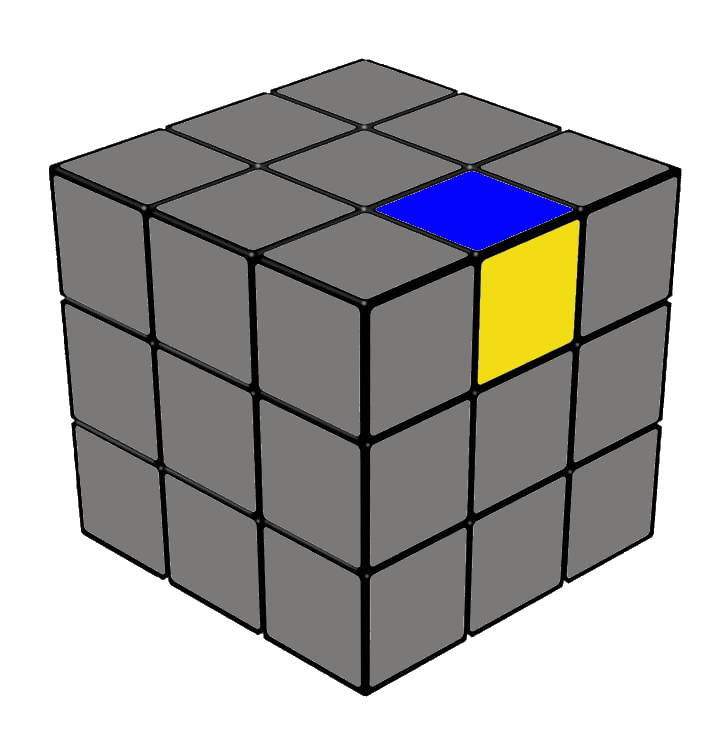
\includegraphics[height=2cm]{images/slozena-ivica.png}
        }
        \subfigure{
            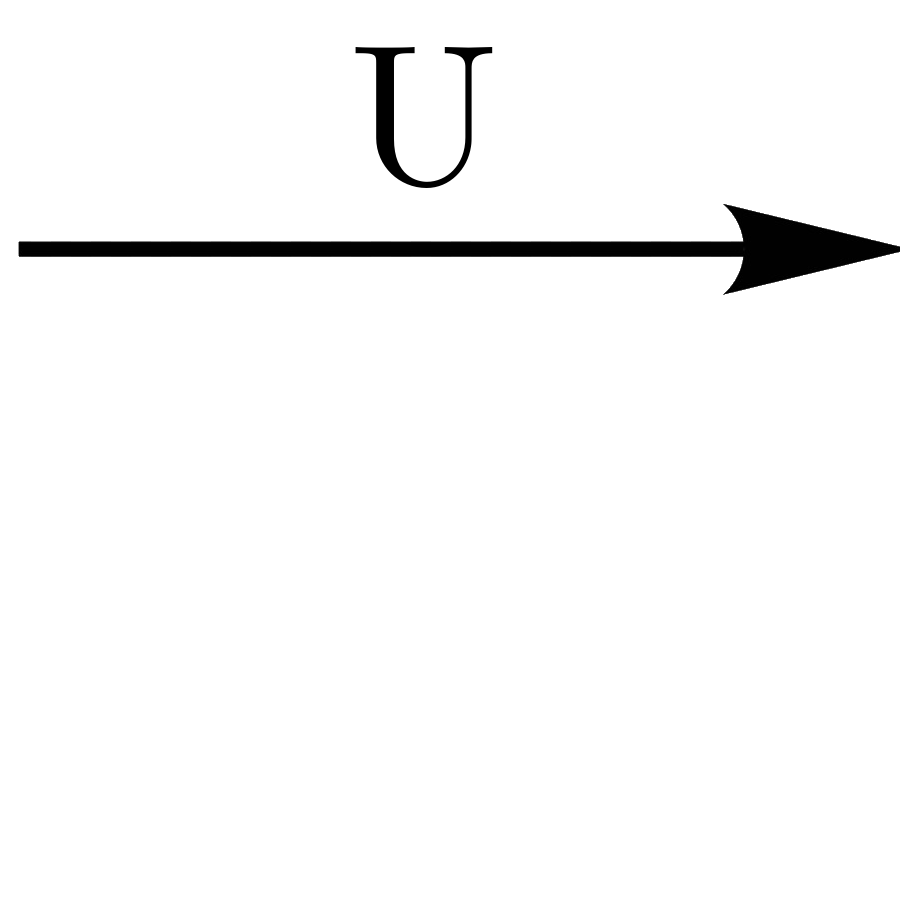
\includegraphics[height=1.5cm]{images/Uarrow.png} 
        }
        \subfigure{
             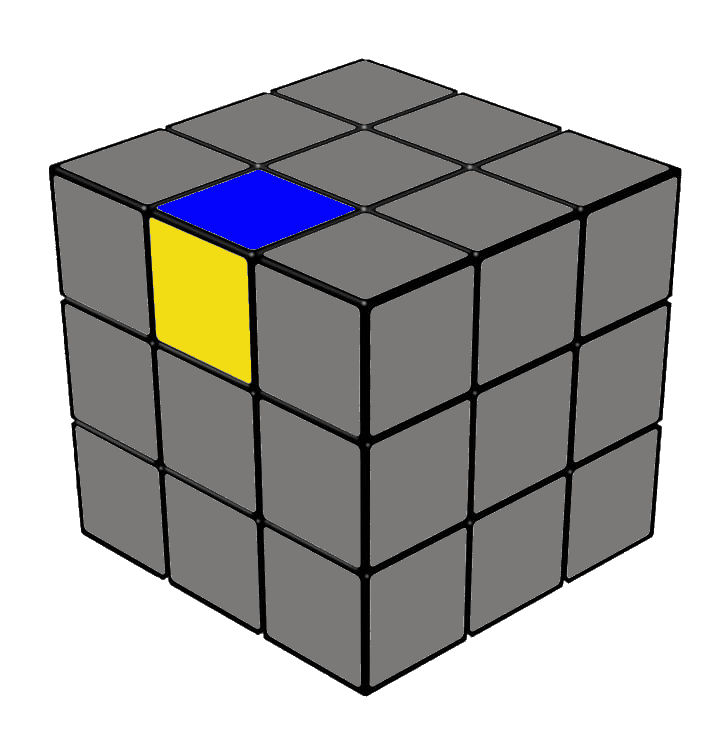
\includegraphics[height=2cm]{images/U-ivica.png}
        }
        \subfigure{
            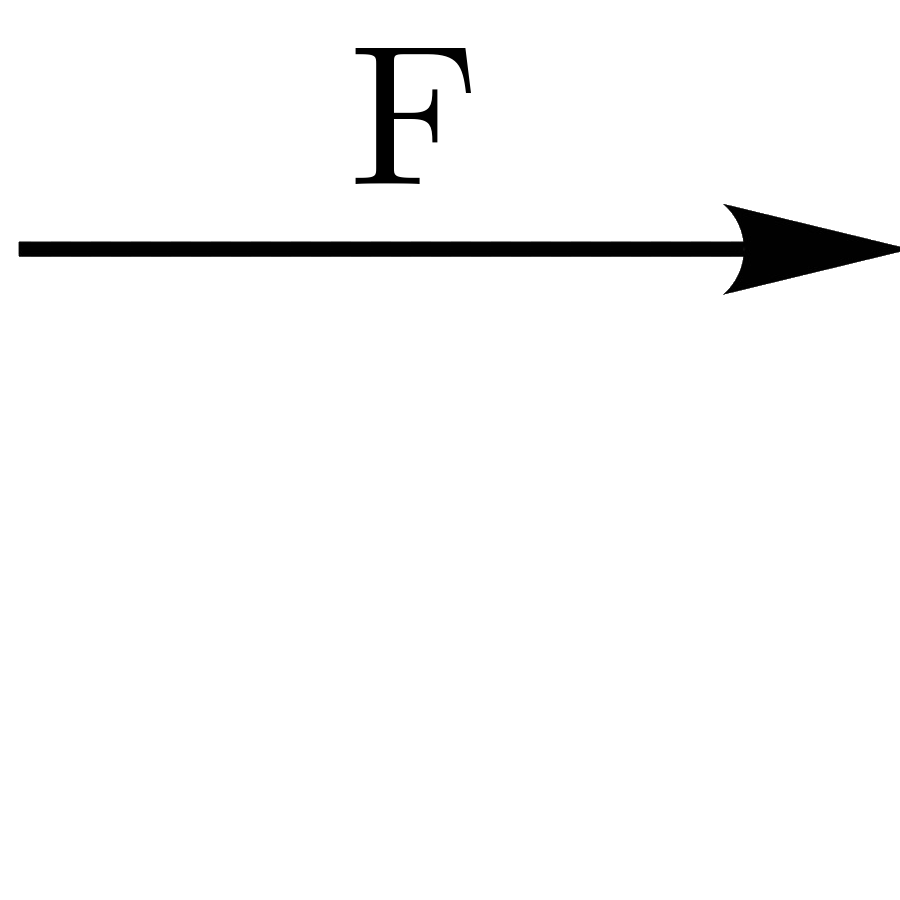
\includegraphics[height=1.5cm]{images/Farrow.png} 
        }
        \subfigure{
             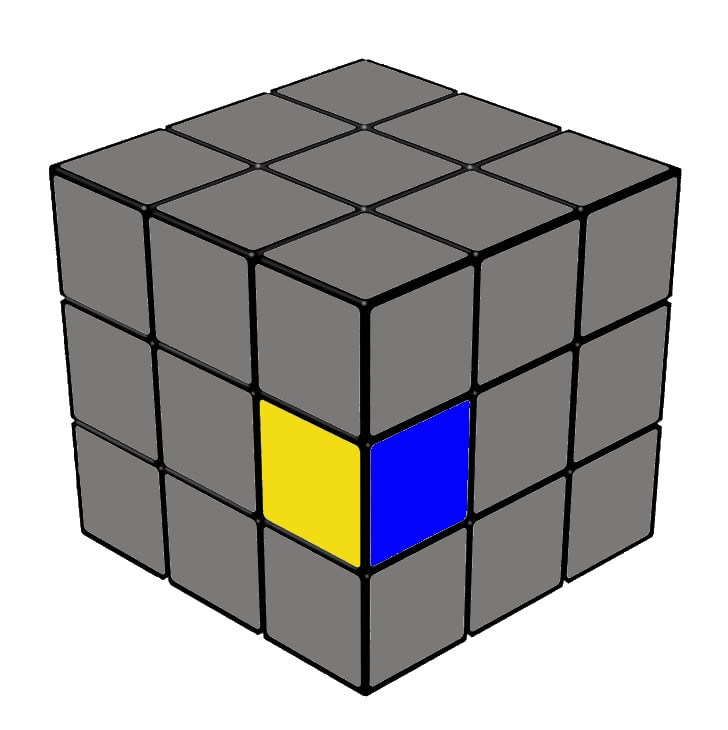
\includegraphics[height=2cm]{images/F-ivica.png}
        }
        \caption{}
        \label{fig:ivica-pomeranje}
    \end{figure}

Zato ivice imaju samo 12 mesta na kojima se mogu naći i jedno stanje kocke može imati samo jednu permutaciju tih ivica. S obzirom da se ivice i ćoškovi razlikuju i njihove permutacije se gledaju odvojeno jedne od drugih.

\begin{primer} I tabele treba da budu u svom okruženju, i na njih je neophodno referisati se u tekstu. Na primer, u tabeli \ref{tab:tabela1} su prikazana različita poravnanja u tabelama.

\begin{table}[h!]
\begin{center}
\caption{Razlčita poravnanja u okviru iste tabele ne treba koristiti jer su nepregledna.}
\begin{tabular}{|c|l|r|} \hline
centralno poravnanje& levo poravnanje& desno poravnanje\\ \hline
a &b&c\\ \hline
d &e&f\\ \hline
\end{tabular}
\label{tab:tabela1}
\end{center}
\end{table}

\end{primer}






\section{Zaključak}
\label{sec:zakljucak}

Ovde pišem zaključak. 
Ovde pišem zaključak. 
Ovde pišem zaključak. 
Ovde pišem zaključak. 
Ovde pišem zaključak. 
Ovde pišem zaključak. 
Ovde pišem zaključak. 
Ovde pišem zaključak. 
Ovde pišem zaključak. 
Ovde pišem zaključak. 
Ovde pišem zaključak. 
Ovde pišem zaključak. 


\addcontentsline{toc}{section}{Literatura}
\appendix

\iffalse
\bibliography{seminarski} 
\bibliographystyle{plain}
\fi

\begin{thebibliography}{9}

\bibitem{laski2009software} J. Laski and W. Stanley. \emph{Software Verification and Analysis}. Springer- Verlag, London, 2009.

\bibitem{gcc} Free Software Foundation. GNU gcc, 2013. on-line at: http://gcc. gnu.org/.

\bibitem{haltingproblem} A. M. Turing. \emph{On Computable Numbers, with an application to the Entscheidungsproblem}. Proceedings of the London Mathematical Society, 2(42):230–265, 1936.


\end{thebibliography}


\appendix
\section{Dodatak}
Ovde pišem dodatne stvari, ukoliko za time ima potrebe.
Ovde pišem dodatne stvari, ukoliko za time ima potrebe.
Ovde pišem dodatne stvari, ukoliko za time ima potrebe.
Ovde pišem dodatne stvari, ukoliko za time ima potrebe.
Ovde pišem dodatne stvari, ukoliko za time ima potrebe.


\end{document}
